\documentclass[aspectratio=169,12pt,t]{beamer}

% --- Theme: Metropolis (modern, clean) ---
\usetheme[progressbar=frametitle,numbering=fraction,block=fill]{metropolis}

% --- Fira Sans font (install texlive-fonts-extra if missing) ---
\IfFileExists{FiraSans.sty}{\usepackage[sfdefault]{FiraSans}}{}

% --- Light background with warm accent ---
\definecolor{mDarkTeal}{RGB}{35,55,59}
\definecolor{mLightBrown}{RGB}{235,228,216}
\definecolor{mAccent}{RGB}{140,70,20}

\setbeamercolor{normal text}{fg=mDarkTeal,bg=white}
\setbeamercolor{alerted text}{fg=mAccent}
\setbeamercolor{frametitle}{bg=mDarkTeal,fg=white}
\setbeamercolor{progress bar}{fg=mAccent,bg=mLightBrown}
\setbeamercolor{title separator}{fg=mAccent}
\setbeamercolor{progress bar in head/foot}{fg=mAccent,bg=mLightBrown}
\setbeamercolor{progress bar in section page}{fg=mAccent,bg=mLightBrown}

% --- Packages ---
\usepackage[utf8]{inputenc}
\usepackage{amsmath,amssymb,amsthm}
\usepackage{mathrsfs}
\usepackage{tikz}
\usetikzlibrary{arrows.meta,positioning,calc,decorations.pathreplacing,shapes,patterns}
\usepackage{pgfplots}
\pgfplotsset{compat=1.18}

% --- Semi-transparent white highlight for text on top of background images ---
\usepackage[most]{tcolorbox}

% Inline highlight: \hl{short text}
\newtcbox{\hl}{%
  nobeforeafter, tcbox raise base,
  colback=white, opacityback=0.6,
  colframe=white, opacityframe=0,
  sharp corners, boxsep=2pt, left=3pt, right=3pt, top=2pt, bottom=2pt%
}

% Block highlight: \begin{hlbox} ... \end{hlbox}  (multi-line, paragraphs, itemize)
\newtcolorbox{hlbox}[1][]{%
  enhanced, breakable,
  colback=white, opacityback=0.6,
  colframe=white, opacityframe=0,
  boxsep=3pt, left=6pt, right=6pt, top=4pt, bottom=4pt,
  sharp corners,
  {#1}%
}

% --- Custom colors for content types ---
\definecolor{defcolor}{RGB}{25,85,120}
\definecolor{thmcolor}{RGB}{140,35,35}
\definecolor{proofcolor}{RGB}{35,100,50}
\definecolor{excolor}{RGB}{140,75,10}
\definecolor{remcolor}{RGB}{90,90,90}

% --- Beamer blocks for mathematical content types (semi-transparent) ---
\tcbset{hlblockbase/.style={
  enhanced, breakable,
  coltitle=white, fonttitle=\bfseries,
  opacitybacktitle=0.8, opacityback=0.6,
  opacityframe=0,
  sharp corners,
  boxsep=1pt, left=5pt, right=5pt, top=2pt, bottom=2pt,
  toptitle=1pt, bottomtitle=1pt
}}

\newtcolorbox{defblock}[1]{hlblockbase, title={#1},
  colbacktitle=defcolor, colback=defcolor!15, colframe=defcolor}
\newtcolorbox{thmblock}[1]{hlblockbase, title={#1},
  colbacktitle=thmcolor, colback=thmcolor!15, colframe=thmcolor}
\newtcolorbox{proofblock}[1]{hlblockbase, title={#1},
  colbacktitle=proofcolor, colback=proofcolor!15, colframe=proofcolor}
\newtcolorbox{exblock}[1]{hlblockbase, title={#1},
  colbacktitle=excolor, colback=excolor!15, colframe=excolor}
\newtcolorbox{remblock}[1]{hlblockbase, title={#1},
  colbacktitle=remcolor, colback=remcolor!15, colframe=remcolor}

% --- Metadata ---
\title{Chapter 3: Numerical Sequences and Series}
\subtitle{Section: Some Special Sequences}
\author{Based on Walter Rudin's \emph{Principles of Mathematical Analysis}}
\date{}

\begin{document}

% =============================================================================
% TITLE AND OUTLINE
% =============================================================================
{
\usebackgroundtemplate{%
  
\includegraphics[width=\paperwidth,height=\paperheight,keepaspectratio=false]{chapter_03_bg_00.png}%
}
\begin{frame}[plain]
  \titlepage
  \note{
    Welcome back to Chapter 3 of Principles of Mathematical Analysis.
    So far we have studied convergent sequences, subsequences, Cauchy
    sequences, and upper and lower limits. In this short but useful
    section we step back from the abstract theory and compute the
    limits of five sequences that show up again and again in analysis.
    The five limits collected in Theorem 3.20 are the workhorses we
    will reach for in the rest of the chapter, especially when we test
    series for convergence. Every proof relies on a single simple
    bounding principle, which we will isolate first and then apply
    five times.
  }
\end{frame}
}

{
\usebackgroundtemplate{%
  
\includegraphics[width=\paperwidth,height=\paperheight,keepaspectratio=false]{chapter_03_bg_01.png}%
}
\begin{frame}[c]{Outline}
  \begin{center}
    \tableofcontents
  \end{center}
  \note{
    Here is the plan. We open with a brief motivation: why these
    particular sequences deserve their own section. We then
    assemble two tools: the squeeze principle, a simple bounding
    remark, and the binomial theorem, which we build up carefully
    and prove. Next we state Theorem 3.20 with its five parts.
    After that we walk through the proofs one by one. Part "a" is
    a direct application of the archimedean property. Parts "b"
    and "c" rely on the binomial theorem. Part "d" extends the
    binomial idea to higher powers, and part "e" is then a
    one-line consequence. We close with a summary and a look ahead
    to series.
  }
\end{frame}

% =============================================================================
% MOTIVATION
% =============================================================================
\section{Motivation}

% --- Build 1/4 ---
\begin{frame}{Why a Section on Special Sequences?}
  \begin{hlbox}
    \begin{itemize}
      \item Theory so far is \alert{abstract} (limits, Cauchy, $\limsup$)
    \end{itemize}
  \end{hlbox}

  \note{
    Up to this point the chapter has been mostly abstract. We
    defined what it means for a sequence to converge, what a Cauchy
    sequence is, what the upper and lower limits are. We have very
    few concrete sequences in our toolkit yet.
  }
\end{frame}

% --- Build 2/4 ---
\begin{frame}{Why a Section on Special Sequences?}
  \begin{hlbox}
    \begin{itemize}
      \item Theory so far is \alert{abstract} (limits, Cauchy, $\limsup$)
      \item Yet a few \emph{concrete} sequences appear \alert{constantly} in analysis
    \end{itemize}
  \end{hlbox}

  \note{
    But certain concrete sequences appear so often that they deserve
    to be in our muscle memory. Expressions like 1 over "n", the "n"
    th root of a constant, the "n" th root of "n", or powers of a
    number less than 1 in absolute value, show up over and over
    again in proofs.
  }
\end{frame}

% --- Build 3/4 ---
\begin{frame}{Why a Section on Special Sequences?}
  \begin{hlbox}
    \begin{itemize}
      \item Theory so far is \alert{abstract} (limits, Cauchy, $\limsup$)
      \item Yet a few \emph{concrete} sequences appear \alert{constantly} in analysis
      \item \alert{Goal:} compute limits of five recurring sequences once and for all
    \end{itemize}
  \end{hlbox}

  \note{
    Our goal in this section is to pin down the limits of five such
    sequences, once and for all. After this short section we will
    treat the answers as known facts and quote them freely. Doing the
    work here, in one place, saves us from repeating the same
    binomial estimates in the chapters to come.
  }
\end{frame}

% --- Build 4/4 ---
\begin{frame}{Why a Section on Special Sequences?}
  \begin{hlbox}
    \begin{itemize}
      \item Theory so far is \alert{abstract} (limits, Cauchy, $\limsup$)
      \item Yet a few \emph{concrete} sequences appear \alert{constantly} in analysis
      \item \alert{Goal:} compute limits of five recurring sequences once and for all
      \item \alert{One technique} powers every proof: a simple \emph{squeeze}
    \end{itemize}
  \end{hlbox}

  \note{
    One more point is worth flagging up front. All five proofs
    share a single tool: a simple squeeze. If we can bound a
    nonnegative sequence above by something that visibly goes to
    zero, then our sequence also goes to zero. That is the entire
    engine. We will isolate it first, and then just apply it five
    times.
  }
\end{frame}
}

{
\usebackgroundtemplate{%
  
\includegraphics[width=\paperwidth,height=\paperheight,keepaspectratio=false]{chapter_03_bg_02.png}%
}
% =============================================================================
% THE SQUEEZE PRINCIPLE
% =============================================================================
\section{The Squeeze Principle}

% --- The squeeze remark ---
\begin{frame}{A Useful Bounding Remark}
  \begin{remblock}{Squeeze to zero}
    If $0 \leq x_n \leq s_n$ for all $n \geq N$, and $s_n \to 0$, then $x_n \to 0$.
  \end{remblock}

  \vspace{0.6em}
  \begin{hlbox}
    \textbf{Why it works:} given $\varepsilon > 0$, eventually $s_n < \varepsilon$, and so
    $\;0 \leq x_n \leq s_n < \varepsilon$.
  \end{hlbox}

  \note{
    Here is the bounding remark in precise form. Suppose we have a
    nonnegative sequence "x" sub "n" that is dominated past some
    index by a sequence "s" sub "n" that we already know goes to
    zero. Then "x" sub "n" also goes to zero.

    The proof is one line. Given any positive epsilon, since "s" sub
    "n" goes to zero we can find an index past which "s" sub "n" is
    less than epsilon. From that index on, our sequence "x" sub "n"
    is squeezed between 0 and epsilon, which is exactly the
    definition of converging to zero.
  }
\end{frame}

% --- Visual: squeeze ---
\begin{frame}{Picture: A Vanishing Envelope}
  \begin{center}
  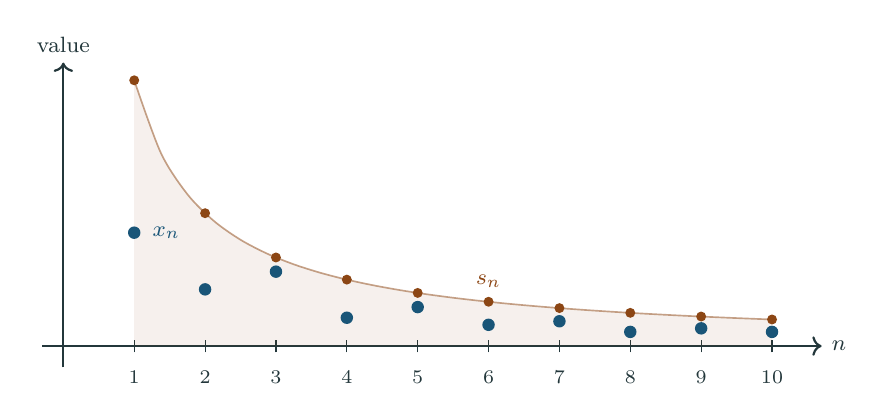
\begin{tikzpicture}[scale=0.9]
    % Axes
    \draw[->, thick, mDarkTeal] (-0.3, 0) -- (10.7, 0) node[right]{\footnotesize $n$};
    \draw[->, thick, mDarkTeal] (0, -0.3) -- (0, 4.0) node[above]{\footnotesize value};
    % x-axis ticks at the integer indices n = 1, 2, 3, ...
    \foreach \n in {1,...,10} {
      \draw[mDarkTeal] (\n, -0.09) -- (\n, 0.09);
      \node[mDarkTeal, below=3pt] at (\n, -0.09) {\scriptsize \n};
    }
    % shading between 0 and s_n
    \fill[mAccent, opacity=0.08] plot[domain=1:10, smooth] (\x, {3.0/(\x*0.8)}) -- (10, 0) -- (1, 0) -- cycle;
    % envelope s_n: faint guide curve through the dots
    \draw[semithick, mAccent, opacity=0.5, domain=1:10, smooth] plot (\x, {3.0/(\x*0.8)});
    % s_n dots (brown): s_n is itself a sequence, not a function
    \foreach \x in {1,...,10} {
      \fill[mAccent] (\x, {3.0/(\x*0.8)}) circle (2pt);
    }
    \node[mAccent] at (6.0, 0.92) {\footnotesize $s_n$};
    % x_n dots, all sitting between 0 and s_n
    \fill[defcolor] (1.0, 1.6) circle (2.5pt);
    \fill[defcolor] (2.0, 0.8) circle (2.5pt);
    \fill[defcolor] (3.0, 1.05) circle (2.5pt);
    \fill[defcolor] (4.0, 0.4) circle (2.5pt);
    \fill[defcolor] (5.0, 0.55) circle (2.5pt);
    \fill[defcolor] (6.0, 0.3) circle (2.5pt);
    \fill[defcolor] (7.0, 0.35) circle (2.5pt);
    \fill[defcolor] (8.0, 0.2) circle (2.5pt);
    \fill[defcolor] (9.0, 0.25) circle (2.5pt);
    \fill[defcolor] (10.0, 0.2) circle (2.5pt);
    \node[defcolor, right] at (1.12, 1.6) {\footnotesize $x_n$};
  \end{tikzpicture}
  \end{center}

  \vspace{0.2em}
  \begin{center}
    \hl{Each $x_n$ is trapped between $0$ and $s_n$.}
  \end{center}

  \note{
    Here is the picture behind the squeeze. The horizontal axis is
    the index "n", and it is now marked with ticks at the whole
    numbers 1, 2, 3, and onward, to stress that we are working with
    a sequence and not a continuous function. The vertical axis is
    the value. The brown dots are the dominating sequence "s" sub
    "n"; the faint brown curve through them is just a visual guide.
    The blue dots are our sequence "x" sub "n". At every index, the
    blue dot lies below the brown dot, inside the shaded band
    between zero and "s" sub "n". As the brown dots collapse onto
    the horizontal axis, the blue dots have nowhere to go but down
    to zero with them. That is the squeeze in one picture. Next we
    gather a second tool, the binomial theorem, which will supply
    the bounds we feed into this squeeze.
  }
\end{frame}

}

{
\usebackgroundtemplate{%
  
\includegraphics[width=\paperwidth,height=\paperheight,keepaspectratio=false]{chapter_03_bg_03.png}%
}
% =============================================================================
% THE BINOMIAL THEOREM (the tool used in the proofs of (b), (c), (d))
% =============================================================================
\section{The Binomial Theorem}

% --- Definition of the factorial ---
\begin{frame}{The Factorial}
  \begin{defblock}{Definition --- Factorial}
    For an integer $n \geq 1$,
    \[
      n! \;=\; n \cdot (n-1) \cdot (n-2) \cdots 2 \cdot 1,
      \qquad\text{and}\qquad 0! = 1 .
    \]
  \end{defblock}

  \vspace{0.5em}
  \begin{thmblock}{What $n!$ counts}
    $n!$ is the number of \alert{permutations} of $\{1, 2, \dots, n\}$: the orderings of
    $n$ distinct objects in a row.
  \end{thmblock}

  \vspace{0.3em}
  \begin{hlbox}
    \textbf{Why:} $n$ choices for the first slot, $n-1$ for the second, \ldots, $1$ for the last.
  \end{hlbox}

  \note{
    The binomial theorem rests on the binomial coefficient, and the
    binomial coefficient is in turn built from factorials, so we
    start at the bottom, with the factorial itself. For a whole
    number "n" at least 1, "n" factorial is the product "n" times
    "n" minus 1 times "n" minus 2, and so on down to 1. By
    convention, 0 factorial is 1.

    Like the binomial coefficient to come, the factorial has a
    counting meaning, shown in the red block: "n" factorial is the
    number of permutations of the set 1 through "n", that is, the
    number of ways to arrange "n" distinct objects in a row. The
    reason is a quick choice count: "n" objects could go in the
    first slot, then "n" minus 1 remain for the second, and so on,
    until a single object is left for the last. Multiplying the
    choices gives "n" factorial.
  }
\end{frame}

% --- Example: permutations of {1,2,3} ---
\begin{frame}{Example: The $3! = 6$ Permutations of $\{1,2,3\}$}
  \begin{center}
  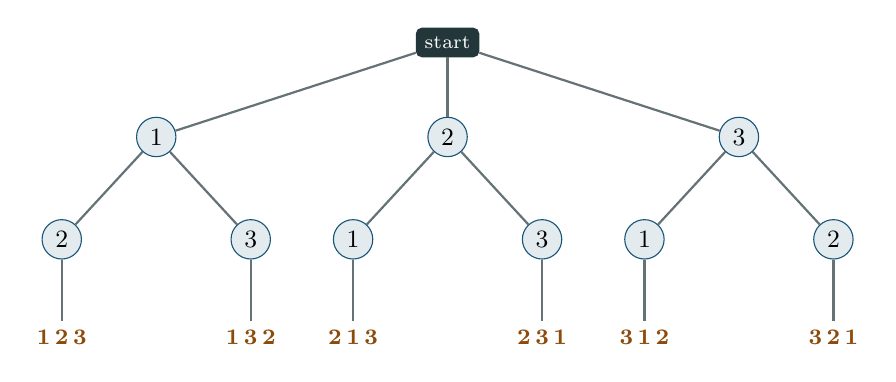
\begin{tikzpicture}[
      every node/.style={font=\footnotesize},
      nd/.style={circle, draw=defcolor, fill=defcolor!12, inner sep=1.6pt,
                 minimum size=5mm, font=\small},
      rt/.style={rectangle, rounded corners=2pt, draw=mDarkTeal, fill=mDarkTeal,
                 text=white, inner sep=3pt, font=\scriptsize},
      lf/.style={font=\footnotesize\bfseries, text=excolor},
      ed/.style={mDarkTeal!70, thick}
    ]
    % root
    \node[rt] (r) at (0, 2.7) {start};
    % level 1: first entry
    \node[nd] (a1) at (-3.7, 1.5) {1};
    \node[nd] (a2) at (0, 1.5) {2};
    \node[nd] (a3) at (3.7, 1.5) {3};
    % level 2: second entry
    \node[nd] (b1) at (-4.9, 0.2) {2};
    \node[nd] (b2) at (-2.5, 0.2) {3};
    \node[nd] (b3) at (-1.2, 0.2) {1};
    \node[nd] (b4) at (1.2, 0.2) {3};
    \node[nd] (b5) at (2.5, 0.2) {1};
    \node[nd] (b6) at (4.9, 0.2) {2};
    % leaves: full permutations (third entry is forced)
    \node[lf] (l1) at (-4.9, -1.05) {1\,2\,3};
    \node[lf] (l2) at (-2.5, -1.05) {1\,3\,2};
    \node[lf] (l3) at (-1.2, -1.05) {2\,1\,3};
    \node[lf] (l4) at (1.2, -1.05) {2\,3\,1};
    \node[lf] (l5) at (2.5, -1.05) {3\,1\,2};
    \node[lf] (l6) at (4.9, -1.05) {3\,2\,1};
    % edges
    \draw[ed] (r) -- (a1);  \draw[ed] (r) -- (a2);  \draw[ed] (r) -- (a3);
    \draw[ed] (a1) -- (b1); \draw[ed] (a1) -- (b2);
    \draw[ed] (a2) -- (b3); \draw[ed] (a2) -- (b4);
    \draw[ed] (a3) -- (b5); \draw[ed] (a3) -- (b6);
    \draw[ed] (b1) -- (l1); \draw[ed] (b2) -- (l2); \draw[ed] (b3) -- (l3);
    \draw[ed] (b4) -- (l4); \draw[ed] (b5) -- (l5); \draw[ed] (b6) -- (l6);
  \end{tikzpicture}
  \end{center}

  \vspace{0.2em}
  \begin{center}
    \begin{hlbox}
      \centering
      From \emph{start}: $3$ ways to pick the first entry, then $2$, then $1$.\\
      Thus $3! = 3 \cdot 2 \cdot 1 =  6$ orderings are the leaves.
    \end{hlbox}
  \end{center}

  \note{
    Let us make this concrete with "n" equal to 3. The slide shows
    a tree of all the permutations of the set 1, 2, 3. Reading from
    the top: the node marked start branches three ways, one for
    each choice of the first entry. From each of those, the tree
    branches two ways, for the two elements still available for the
    second entry. Finally only one element is left, and it fills
    the third entry, so the bottom row, in amber, lists the six
    complete arrangements. Counting the branches level by level, 3
    times 2 times 1 equals 3 factorial, which is 6. So there are
    exactly six ways to order three objects, just as the formula
    predicts.
  }
\end{frame}

% --- Definition of the binomial coefficient ---
\begin{frame}{The Binomial Coefficient}
  \begin{defblock}{Definition --- Binomial Coefficient}
    For integers $0 \leq k \leq n$,
    \[
      \binom{n}{k} \;=\; \frac{n (n - 1) \cdots (n - k + 1)}{k!} \;=\; \frac{n!}{k!\,(n-k)!}.
    \]
  \end{defblock}

  \vspace{0.5em}
  \begin{thmblock}{What $\binom{n}{k}$ counts}
    $\binom{n}{k}$ is the number of $k$-element subsets of $\{1, \dots, n\}$.
  \end{thmblock}

  \note{
    With the factorial defined, we can introduce the binomial
    coefficient. By definition, "n" choose "k" is a product of "k"
    consecutive integers, "n" times "n" minus 1, down to "n" minus
    "k" plus 1, all divided by "k" factorial. As the slide shows,
    this equals "n" factorial over "k" factorial times "n" minus
    "k" factorial. Either way, the formula carries a concrete
    meaning, stated in the red block: "n" choose "k" is exactly the
    number of "k" element subsets you can form from a set of "n"
    things. On the next slide we prove that the formula and this
    meaning agree, using a counting argument.
  }
\end{frame}

% --- Proof that C(n,k) counts k-element subsets ---
\begin{frame}{Why $\binom{n}{k}$ Counts $k$-Element Subsets}
  \begin{hlbox}
    \textbf{Strategy:} count the ordered $k$-tuples of \emph{distinct} elements of $\{1,\dots,n\}$ in two ways. Let $C$ be the number of $k$-element subsets.
  \end{hlbox}

  \vspace{0.4em}
  \begin{proofblock}{Two counts of the same collection}
    \begin{enumerate}
      \item \textbf{Directly:} $n$ choices for the first entry, $n-1$ for the second, \ldots, $n-k+1$ for the last:
        $\;n(n-1)\cdots(n-k+1) = \dfrac{n!}{(n-k)!}$ tuples.
      \item \textbf{By grouping:} each $k$-element subset can be ordered in $k!$ ways, giving $\;C \cdot k!$ tuples.
      \item \textbf{Equate:} $\;C \cdot k! = \dfrac{n!}{(n-k)!}$, \;so $\;C = \dfrac{n!}{k!\,(n-k)!} = \binom{n}{k}$. \quad $\Box$
    \end{enumerate}
  \end{proofblock}

  \note{
    Here is the counting argument. We count one and the same
    collection, the ordered "k" tuples of distinct elements drawn
    from the numbers 1 through "n", in two different ways. Write
    "C" for the number of "k" element subsets; that is the quantity
    we want to identify.

    First, count the tuples directly. There are "n" choices for the
    first entry, then "n" minus 1 for the second, since one element
    is now used up, and so on down to "n" minus "k" plus 1 for the
    last entry. Multiplying these gives "n" factorial over "n"
    minus "k" factorial.

    Second, count the tuples by grouping. Every tuple comes from
    choosing a "k" element subset and then ordering it. There are
    "C" subsets, and each can be ordered in "k" factorial ways, so
    this count is "C" times "k" factorial.

    The two counts describe the same collection, so they are equal.
    Dividing by "k" factorial isolates "C", and it equals "n"
    factorial divided by "k" factorial times "n" minus "k"
    factorial, which is exactly "n" choose "k". The formula and the
    meaning agree. The next slide works through a concrete case.
  }
\end{frame}

% --- Example: why C(4,2) counts the 2-element subsets ---
\begin{frame}{Example: $\binom{4}{2}$ Counts the $2$-Subsets of $\{1,2,3,4\}$}
  \begin{hlbox}
    \textbf{Count the ordered pairs of distinct elements two ways:}\\
    Directly, $4 \cdot 3 = 12$; \;or as $(\#\text{ subsets}) \times 2!$.
  \end{hlbox}

  \vspace{0.5em}
  \begin{center}
  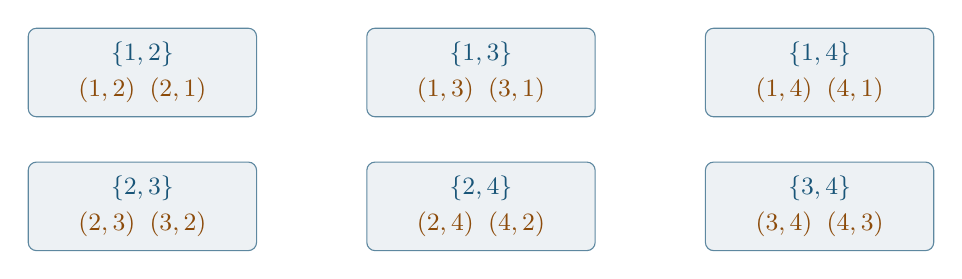
\begin{tikzpicture}[
      box/.style={rectangle, rounded corners=3pt, draw=defcolor!70, fill=defcolor!8,
                  inner sep=5pt, align=center, minimum width=2.9cm, font=\small}
    ]
    \node[box] at (-4.3,  0.0) {{\color{defcolor}\bfseries$\{1,2\}$}\\[2pt]{\color{excolor}$(1,2)\;\;(2,1)$}};
    \node[box] at ( 0.0,  0.0) {{\color{defcolor}\bfseries$\{1,3\}$}\\[2pt]{\color{excolor}$(1,3)\;\;(3,1)$}};
    \node[box] at ( 4.3,  0.0) {{\color{defcolor}\bfseries$\{1,4\}$}\\[2pt]{\color{excolor}$(1,4)\;\;(4,1)$}};
    \node[box] at (-4.3, -1.7) {{\color{defcolor}\bfseries$\{2,3\}$}\\[2pt]{\color{excolor}$(2,3)\;\;(3,2)$}};
    \node[box] at ( 0.0, -1.7) {{\color{defcolor}\bfseries$\{2,4\}$}\\[2pt]{\color{excolor}$(2,4)\;\;(4,2)$}};
    \node[box] at ( 4.3, -1.7) {{\color{defcolor}\bfseries$\{3,4\}$}\\[2pt]{\color{excolor}$(3,4)\;\;(4,3)$}};
  \end{tikzpicture}
  \end{center}

  \vspace{0.3em}
  \begin{center}
    \hl{Each subset accounts for $2! = 2$ ordered pairs, so $\;\binom{4}{2} = \dfrac{12}{2!} = 6$.}
  \end{center}

  \note{
    Let us see the counting proof in action, with "n" equal to 4
    and "k" equal to 2. We want the number of 2 element subsets of
    the set 1 through 4. Following the proof, we count the ordered
    pairs of distinct elements two ways.

    Counting directly, there are 4 choices for the first entry and
    3 for the second, giving 12 ordered pairs; that is 4 factorial
    over 2 factorial. The slide groups those same 12 pairs into 6
    boxes, one box per 2 element subset. Each subset, shown in
    blue, sits above its 2 orderings, shown in amber: for instance
    the subset containing 1 and 2 accounts for the pair 1 then 2,
    and the pair 2 then 1.

    Since every subset contributes exactly 2 factorial, which is 2,
    ordered pairs, the number of subsets is 12 divided by 2
    factorial, which is 6. And 6 is exactly 4 choose 2. The general
    formula and the concrete count agree.
  }
\end{frame}

% --- Statement ---
\begin{frame}{The Binomial Theorem}
  \begin{thmblock}{Binomial Theorem}
    For all real $a, b$ and every integer $n \geq 0$,
    \[
      (a + b)^n \;=\; \sum_{k=0}^{n} \binom{n}{k}\, a^{n-k} b^k.
    \]
  \end{thmblock}

  \vspace{0.25em}
  \begin{hlbox}
    {\small We take $0^0 = 1$ for notational simplicity (in general, $0^0$ is undefined).}
  \end{hlbox}

  \note{
    With the binomial coefficient defined and understood, we can
    state the binomial theorem itself. It expands a power of a sum:
    "a" plus "b", raised to the "n" th power, becomes a sum of "n"
    plus 1 terms, and the "k" th term is the binomial coefficient
    "n" choose "k", which we just studied, times "a" to the "n"
    minus "k", times "b" to the "k".

    One small notational point. When "a" or "b" is zero, the
    formula produces a term with zero raised to the zero power,
    which is normally left undefined. Throughout the binomial
    theorem we simply adopt the convention that zero to the zero
    power equals 1. That keeps every term meaningful and the
    formula correct even in boundary cases, such as "a" plus zero
    raised to the "n" th power, which should of course equal "a"
    to the "n".
  }
\end{frame}

% --- Pascal's rule: counting proof (its own slide) ---
\begin{frame}{Pascal's Rule --- A Counting Proof}
  \begin{remblock}{Pascal's Rule}
    \[
      \binom{n+1}{k} = \binom{n}{k} + \binom{n}{k-1},\quad 1 \leq k \leq n.
    \]
  \end{remblock}

  \vspace{0.4em}
  \begin{proofblock}{Proof by counting}
    $\binom{n+1}{k}$ is the number of $k$-element subsets of $\{1, \dots, n+1\}$.
    Split these subsets by whether or not they contain the element $n+1$:
    \begin{itemize}
      \item \alert{without} $n+1$: a $k$-subset of $\{1,\dots,n\}$, so $\binom{n}{k}$ of them;
      \item \alert{with} $n+1$: the element $n+1$ adjoined to a $(k-1)$-subset of $\{1,\dots,n\}$, so $\binom{n}{k-1}$ of them.
    \end{itemize}
    The two cases are disjoint and exhaustive, so
    $\;\binom{n+1}{k} = \binom{n}{k} + \binom{n}{k-1}$. \quad $\Box$
  \end{proofblock}

  \note{
    One identity our induction proof will lean on is Pascal's
    rule: "n" plus 1 choose "k" equals "n" choose "k", plus "n"
    choose "k" minus 1. Here is a short counting proof.

    The left side, "n" plus 1 choose "k", counts the "k" element
    subsets of the whole numbers 1 through "n" plus 1. We sort
    those subsets into two piles by whether or not they contain
    the largest number, "n" plus 1. A subset that leaves "n" plus
    1 out is simply a "k" element subset of 1 through "n", and
    there are "n" choose "k" of those. A subset that includes "n"
    plus 1 is that number adjoined to a "k" minus 1 element subset
    of 1 through "n", and there are "n" choose "k" minus 1 of
    those. The two piles are disjoint and together account for
    every subset, so adding their counts gives "n" choose "k" plus
    "n" choose "k" minus 1. That is Pascal's rule.
  }
\end{frame}

% --- Proof: Build 1/3 (base + inductive step: the two sums) ---
\begin{frame}{The Binomial Theorem --- Proof by Induction}
  \begin{hlbox}
    \textbf{Induction on $n$.} \;\emph{Base} ($n = 0$): $(a+b)^0 = 1$. \;\emph{Step:} assume it holds for $n$.
  \end{hlbox}

  \vspace{0.3em}
  \begin{proofblock}{Steps}
    \begin{enumerate}
      \item \textbf{Multiply} $(a+b)^n = \sum_{k=0}^{n} \binom{n}{k}\, a^{n-k} b^k$ \textbf{by} $(a+b)$:
        $(a+b)^{n+1} = \left[ \sum_{k=0}^{n} \binom{n}{k}\, a^{n+1-k} b^k \right]
        + \left[ \sum_{k=0}^{n} \binom{n}{k}\, a^{n-k} b^{k+1} \right].$
    \end{enumerate}
  \end{proofblock}

  \note{
    We prove the binomial theorem by induction on "n". The base
    case is "n" equals 0: both sides are simply 1, so the formula
    holds.

    For the inductive step, assume the formula holds for some "n".
    To reach "n" plus 1, we write "a" plus "b" to the "n" plus 1 as
    "a" plus "b", times "a" plus "b" to the "n", and substitute the
    inductive hypothesis. Multiplying that sum through by "a", and
    separately by "b", produces the two sums on the slide. In the
    left sum every power of "a" has gone up by one; in the right
    sum every power of "b" has gone up by one. Next we line these
    two sums up term by term.
  }
\end{frame}

% --- Proof: Build 2/3 (reindex + the two endpoint terms) ---
\begin{frame}{The Binomial Theorem --- Proof by Induction}
  \begin{hlbox}
    \textbf{Induction on $n$.} \;\emph{Base} ($n = 0$): $(a+b)^0 = 1$. \;\emph{Step:} assume it holds for $n$.
  \end{hlbox}

  \vspace{0.3em}
  \begin{proofblock}{Steps}
    \begin{enumerate}
      \item \textbf{Multiply} $(a+b)^n = \sum_{k=0}^{n} \binom{n}{k}\, a^{n-k} b^k$ \textbf{by} $(a+b)$:
        $(a+b)^{n+1} = \left[ \sum_{k=0}^{n} \binom{n}{k}\, a^{n+1-k} b^k \right]
        + \left[ \sum_{k=0}^{n} \binom{n}{k}\, a^{n-k} b^{k+1} \right].$
      \vspace{0.3em}

      Reindex the right sum by $k \mapsto k-1$ (now $k = 1, \dots, n+1$).
      $(a+b)^{n+1} = \left[ \sum_{k=0}^{n} \binom{n}{k}\, a^{n+1-k} b^k \right]
        + \left[ \sum_{k=1}^{n+1} \binom{n}{k-1}\, a^{n+1-k} b^k \right].$
      \item \textbf{Endpoint terms}
        \begin{itemize}
          \item $k = 0$ (left sum): $\;\binom{n}{0} a^{n+1} = \binom{n+1}{0} a^{n+1}$, since $\binom{n}{0} = \binom{n+1}{0} = 1$.
          \item $k = n+1$ (right sum): $\;\binom{n}{n} b^{n+1} = \binom{n+1}{n+1} b^{n+1}$, since $\binom{n}{n} = \binom{n+1}{n+1} = 1$.
        \end{itemize}
    \end{enumerate}
  \end{proofblock}

  \note{
    Now we collect, for each "k", the coefficient of "a" to the "n"
    plus 1 minus "k", times "b" to the "k". First we reindex the
    right sum, replacing "k" by "k" minus 1, so that it runs over
    "k" from 1 up to "n" plus 1.

    Two terms sit at the ends and come from one sum only. At "k"
    equals 0, only the left sum contributes; its term is "n" choose
    0 times "a" to the "n" plus 1. Since "n" choose 0 and "n" plus
    1 choose 0 are both equal to 1, that coefficient already equals
    "n" plus 1 choose 0. At "k" equals "n" plus 1, only the right
    sum contributes; its term is "n" choose "n" times "b" to the
    "n" plus 1. Since "n" choose "n" and "n" plus 1 choose "n" plus
    1 are both 1, that coefficient already equals "n" plus 1 choose
    "n" plus 1. So both endpoint coefficients are already in the
    form we want.
  }
\end{frame}

% --- Proof: Build 3/3 (middle terms via Pascal + conclude) ---
\begin{frame}{The Binomial Theorem --- Proof by Induction}
  \begin{hlbox}
    \textbf{Induction on $n$.} \;\emph{Base} ($n = 0$): $(a+b)^0 = 1$. \;\emph{Step:} assume it holds for $n$.
  \end{hlbox}

  \vspace{0.3em}
  \begin{proofblock}{Steps}
    \begin{enumerate}
      \item \textbf{Multiply} $(a+b)^n = \sum_{k=0}^{n} \binom{n}{k}\, a^{n-k} b^k$ \textbf{by} $(a+b)$:
        $(a+b)^{n+1} = \left[ \sum_{k=0}^{n} \binom{n}{k}\, a^{n+1-k} b^k \right]
        + \left[ \sum_{k=1}^{n+1} \binom{n}{k-1}\, a^{n+1-k} b^k \right].$
      \item \textbf{Endpoint terms}: $\;\binom{n}{0} a^{n+1} = \binom{n+1}{0} a^{n+1}$. \quad
        $\;\binom{n}{n} b^{n+1} = \binom{n+1}{n+1} b^{n+1}$.
      \item \textbf{Middle terms} ($1 \leq k \leq n$): both sums contribute, so the coefficient at $a^{n+1-k} b^k$ is $\binom{n}{k} + \binom{n}{k-1}$, which equals $\binom{n+1}{k}$ by \alert{Pascal's rule}.
      \item \textbf{Together}
        $(a+b)^{n+1} = \sum_{k=0}^{n+1} \binom{n+1}{k}\, a^{n+1-k} b^k. \;\;\Box$
    \end{enumerate}
  \end{proofblock}

  \note{
    The remaining terms are the middle ones, where "k" runs from 1
    to "n". For each such "k", both sums contribute: the left sum
    with coefficient "n" choose "k", and the reindexed right sum
    with coefficient "n" choose "k" minus 1. Pascal's rule says
    these add up to "n" plus 1 choose "k". So at the endpoints and
    in the middle alike, every coefficient equals "n" plus 1 choose
    "k". The two sums have collapsed into the single binomial
    formula with "n" replaced by "n" plus 1, which closes the
    induction. The binomial theorem is proved. The next slide
    records a second proof, a purely combinatorial one, that is
    worth seeing.
  }
\end{frame}

% --- Remark: combinatorial proof of the binomial theorem ---
\begin{frame}{Remark: A Combinatorial Proof}
  \begin{hlbox}
    Write $(a+b)^n = (a+b)(a+b)\cdots(a+b)$. Expanding the product, each term picks one
    letter, $a$ or $b$, from every factor.
  \end{hlbox}

  \vspace{0.15em}
  \begin{center}
  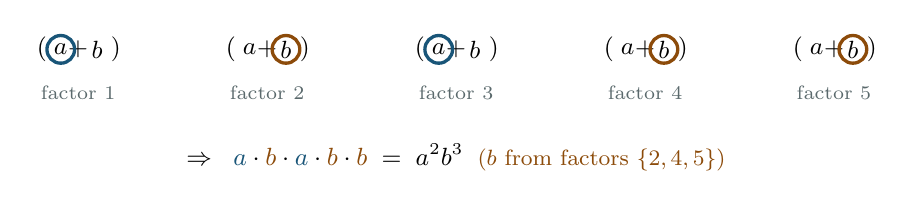
\begin{tikzpicture}[
      every node/.style={font=\small},
      apick/.style={draw=defcolor, very thick},
      bpick/.style={draw=excolor, very thick},
      fnum/.style={font=\scriptsize, text=mDarkTeal!75}
    ]
    \foreach \i/\x in {1/-4.8, 2/-2.4, 3/0, 4/2.4, 5/4.8} {
      \node at (\x-0.46, 0.95) {$($};
      \node (a\i) at (\x-0.22, 0.95) {$a$};
      \node at (\x, 0.95) {$+$};
      \node (b\i) at (\x+0.24, 0.95) {$b$};
      \node at (\x+0.48, 0.95) {$)$};
      \node[fnum] at (\x, 0.40) {factor \i};
    }
    \draw[apick] (a1) circle (5pt);
    \draw[bpick] (b2) circle (5pt);
    \draw[apick] (a3) circle (5pt);
    \draw[bpick] (b4) circle (5pt);
    \draw[bpick] (b5) circle (5pt);
    \node at (0, -0.42) {$\Rightarrow\;\;
      {\color{defcolor}a}\cdot{\color{excolor}b}\cdot{\color{defcolor}a}\cdot{\color{excolor}b}\cdot{\color{excolor}b}
      \;=\; a^{2} b^{3}$\;\;{\footnotesize\color{excolor}($b$ from factors $\{2,4,5\}$)}};
  \end{tikzpicture}
  \end{center}

  \vspace{0.1em}
  \begin{remblock}{Why the coefficient of $a^{n-k} b^k$ is $\binom{n}{k}$}
    In the picture $b$ comes from the $3$-subset $\{2,4,5\}$, giving the term $a^2 b^3$.
    \alert{All $\binom{5}{3} = 10$} of the $3$-subsets give $a^2 b^3$. In general, $b$ from a
    $k$-subset of $\{1,\dots,n\}$ gives $a^{n-k}b^k$, so $(a+b)^n = \sum_{k=0}^{n} \binom{n}{k}\, a^{n-k} b^k$.
  \end{remblock}

  \note{
    Besides the induction, the binomial theorem has a slick
    combinatorial proof. Write "a" plus "b" to the "n" th power as
    a product of "n" copies of "a" plus "b". Multiplying out,
    every term pulls one letter, "a" or "b", from each factor.

    The diagram shows the case "n" equals 5. The five factors are
    in a row, numbered 1 through 5. For one term, the chosen
    letter in each factor is circled: "a" from factors 1 and 3, in
    blue, and "b" from factors 2, 4, and 5, in amber. Multiplying
    the circled letters gives "a" squared times "b" cubed. The
    letter "b" was taken from the factor set containing 2, 4, and
    5.

    Here is the punch line. A term equals "a" squared times "b"
    cubed exactly when "b" is chosen from 3 of the 5 factors, that
    is, from a 3 element subset of 1 through 5. There are 5 choose
    3, or 10, such subsets, so that is the coefficient of "a"
    squared times "b" cubed. The same reasoning, with "k" factors
    giving "b", shows the coefficient of "a" to the "n" minus "k",
    times "b" to the "k", is "n" choose "k", which is the binomial
    theorem. With both tools in hand, the squeeze principle and
    the binomial theorem, we are ready to state the five special
    limits.
  }
\end{frame}

}

{
\usebackgroundtemplate{%
  
\includegraphics[width=\paperwidth,height=\paperheight,keepaspectratio=false]{chapter_03_bg_04.png}%
}
% =============================================================================
% THEOREM 3.20 STATEMENT
% =============================================================================
\section{Five Special Limits}

% --- Build 1/5: part (a) ---
\begin{frame}{Theorem 3.20: Five Special Limits}
  \begin{thmblock}{Theorem 3.20}
    \begin{itemize}
      \item[(a)] If $p > 0$, then $\displaystyle\lim_{n \to \infty} \frac{1}{n^p} = 0$.
    \end{itemize}
  \end{thmblock}

  \note{
    Now we reach the main result of the section. Theorem 3.20
    collects five limits, and we will build the statement one part
    at a time so we can talk about each.

    Part "a" says: if "p" is any positive real number, then 1 over
    "n" to the "p" goes to zero as "n" goes to infinity. For "p"
    equal to 1 this is the familiar fact that 1 over "n" tends to
    zero. The theorem extends it to any positive power, including
    fractional powers like one half, where the sequence is 1 over
    the square root of "n".
  }
\end{frame}

% --- Build 2/5: + part (b) ---
\begin{frame}{Theorem 3.20: Five Special Limits}
  \begin{thmblock}{Theorem 3.20}
    \begin{itemize}
      \item[(a)] If $p > 0$, then $\displaystyle\lim_{n \to \infty} \frac{1}{n^p} = 0$.
      \item[(b)] If $p > 0$, then $\displaystyle\lim_{n \to \infty} \sqrt[n]{p} = 1$.
    \end{itemize}
  \end{thmblock}

  \note{
    Part "b" says: the "n" th root of any positive real number tends
    to 1. So the cube root of 2, the tenth root of 2, the hundredth
    root of 2, and so on, march steadily toward 1 from above; and
    the same is true from below if we start with a positive number
    less than 1. This is a surprising fact when you first meet it,
    because the "n" th root of, say, a million still ends up close
    to 1 once "n" is large enough.
  }
\end{frame}

% --- Build 3/5: + part (c) ---
\begin{frame}{Theorem 3.20: Five Special Limits}
  \begin{thmblock}{Theorem 3.20}
    \begin{itemize}
      \item[(a)] If $p > 0$, then $\displaystyle\lim_{n \to \infty} \frac{1}{n^p} = 0$.
      \item[(b)] If $p > 0$, then $\displaystyle\lim_{n \to \infty} \sqrt[n]{p} = 1$.
      \item[(c)] $\displaystyle\lim_{n \to \infty} \sqrt[n]{n} = 1$.
    \end{itemize}
  \end{thmblock}

  \note{
    Part "c" is even more striking. It says: the "n" th root of "n"
    itself tends to 1. Here the input is no longer a fixed positive
    number but the index "n", which is growing without bound. Even
    so, the "n" th root grows slowly enough to stay arbitrarily
    close to 1. This is one of the most useful concrete limits in
    analysis, and it underpins the root test we will see in a few
    sections.
  }
\end{frame}

% --- Build 4/5: + part (d) ---
\begin{frame}{Theorem 3.20: Five Special Limits}
  \begin{thmblock}{Theorem 3.20}
    \begin{itemize}
      \item[(a)] If $p > 0$, then $\displaystyle\lim_{n \to \infty} \frac{1}{n^p} = 0$.
      \item[(b)] If $p > 0$, then $\displaystyle\lim_{n \to \infty} \sqrt[n]{p} = 1$.
      \item[(c)] $\displaystyle\lim_{n \to \infty} \sqrt[n]{n} = 1$.
      \item[(d)] If $p > 0$ and $\alpha \in \mathbb{R}$, then $\displaystyle\lim_{n \to \infty} \frac{n^\alpha}{(1+p)^n} = 0$.
    \end{itemize}
  \end{thmblock}

  \note{
    Part "d" is the most powerful of the five. It says that any
    polynomial-style growth in "n", written as "n" to the power
    alpha for any real alpha, is eventually crushed by exponential
    growth in the denominator, written as 1 plus "p" raised to the
    "n" th power, whenever "p" is positive. In short, exponentials
    beat polynomials. Note that alpha is allowed to be any real
    number, so even huge powers like "n" to the millionth are
    eventually dominated.
  }
\end{frame}

% --- Build 5/5: + part (e) ---
\begin{frame}{Theorem 3.20: Five Special Limits}
  \begin{thmblock}{Theorem 3.20}
    \begin{itemize}
      \item[(a)] If $p > 0$, then $\displaystyle\lim_{n \to \infty} \frac{1}{n^p} = 0$.
      \item[(b)] If $p > 0$, then $\displaystyle\lim_{n \to \infty} \sqrt[n]{p} = 1$.
      \item[(c)] $\displaystyle\lim_{n \to \infty} \sqrt[n]{n} = 1$.
      \item[(d)] If $p > 0$ and $\alpha \in \mathbb{R}$, then $\displaystyle\lim_{n \to \infty} \frac{n^\alpha}{(1+p)^n} = 0$.
      \item[(e)] If $|x| < 1$, then $\displaystyle\lim_{n \to \infty} x^n = 0$.
    \end{itemize}
  \end{thmblock}

  \note{
    Part "e" rounds out the list. It says that any number "x" whose
    absolute value is strictly less than 1 has powers that tend to
    zero. For example, one half to the "n" goes to zero, and so does
    minus 0.9 to the "n". This is the geometric decay we will lean
    on heavily when we start studying series. As we will see, part
    "e" falls out of part "d" with almost no work.
  }
\end{frame}

}

{
\usebackgroundtemplate{%
  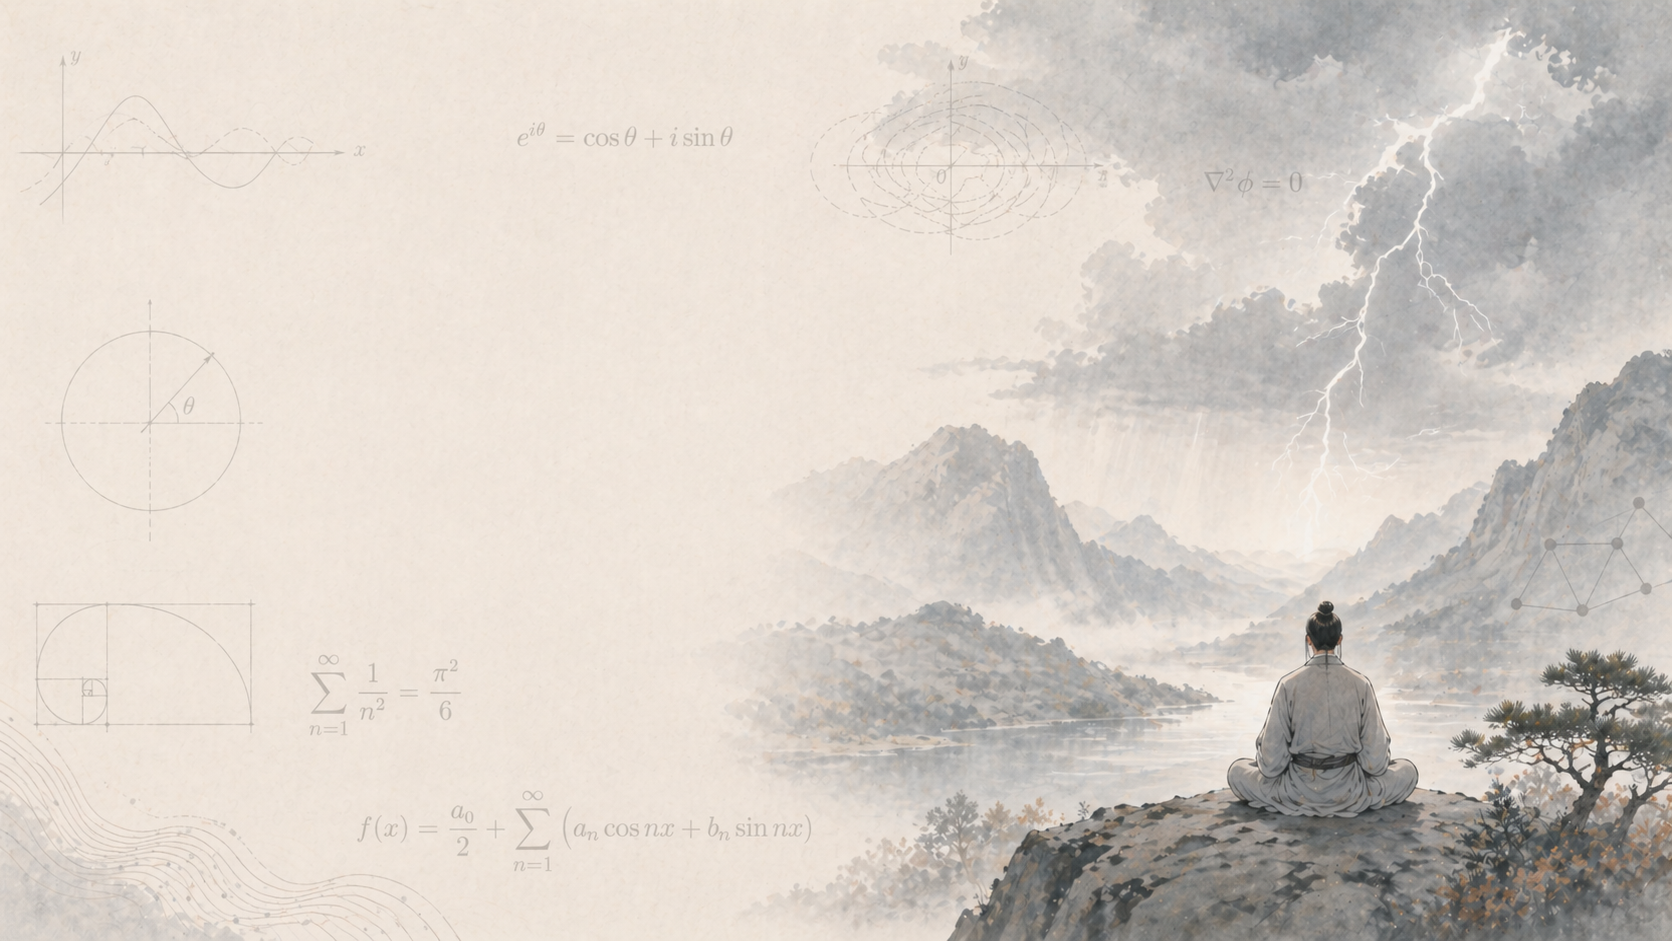
\includegraphics[width=\paperwidth,height=\paperheight,keepaspectratio=false]{chapter_03_bg_05.png}%
}
% =============================================================================
% PROOFS
% =============================================================================
\section{Proofs of the Five Limits}

% --- Proof of (a): Build 1/2 ---
\begin{frame}{Proof of (a): $1/n^p \to 0$}
  \begin{proofblock}{Step 1: Pick a threshold using the archimedean property}
    Fix $\varepsilon > 0$. Choose $n$ large enough that
    \[
      n > \left(\frac{1}{\varepsilon}\right)^{1/p}.
    \]
  \end{proofblock}

  \note{
    We want to show that for every positive epsilon we can find an
    index past which 1 over "n" to the "p" is less than epsilon. To
    arrange this, we solve the inequality 1 over "n" to the "p" is
    less than epsilon for "n", obtaining "n" greater than 1 over
    epsilon, all raised to the power 1 over "p". The archimedean
    property of the real numbers, recalled from Chapter 1, says that
    such an "n" exists no matter how large the right hand side is.
  }
\end{frame}

% --- Proof of (a): Build 2/2 ---
\begin{frame}{Proof of (a): $1/n^p \to 0$}
  \begin{proofblock}{Step 1: Pick a threshold using the archimedean property}
    Fix $\varepsilon > 0$. Choose $n$ large enough that
    $n > (1/\varepsilon)^{1/p}$.
  \end{proofblock}

  \begin{proofblock}{Step 2: Raise to the $p$-th power and rearrange}
    Then $n^p > 1/\varepsilon$, so $\displaystyle\frac{1}{n^p} < \varepsilon$. \quad $\Box$
  \end{proofblock}

  \note{
    Once we have an index "n" exceeding that threshold, raising both
    sides of the inequality to the power "p" gives "n" to the "p"
    greater than 1 over epsilon. Taking reciprocals flips the
    inequality, so 1 over "n" to the "p" is less than epsilon. That
    is precisely what we needed, so the limit is zero.
  }
\end{frame}

% --- Proof of (b): Build 1/3 (case p > 1, setup + step 1) ---
\begin{frame}{Proof of (b): $\sqrt[n]{p} \to 1$ --- Case $p > 1$}
  \begin{hlbox}
    \textbf{Setup.} Put $x_n = \sqrt[n]{p} - 1$. Since $p > 1$, $x_n > 0$ and $\sqrt[n]{p} = 1 + x_n$.
  \end{hlbox}

  \vspace{0.4em}
  \begin{proofblock}{Steps}
    \begin{enumerate}
      \item \textbf{Binomial bound.} $p = (1 + x_n)^n \geq 1 + n x_n$.
    \end{enumerate}
  \end{proofblock}

  \vspace{0.2em}
  \begin{remblock}{Why $(1+x)^n \geq 1 + nx$ for $x \geq 0$ \;(Bernoulli's inequality)}
    The binomial theorem gives $(1+x)^n = 1 + nx + \binom{n}{2} x^2 + \cdots + x^n$,
    a sum of nonnegative terms when $x \geq 0$. Dropping all but the first two terms
    leaves the stated bound.
  \end{remblock}

  \note{
    The strategy is to write the "n" th root of "p" as 1 plus a
    small correction "x" sub "n", and then show that the correction
    shrinks to zero. We begin with the case "p" greater than 1, so
    "x" sub "n" is strictly positive.

    Step 1 is the key estimate: 1 plus "x" sub "n", raised to the
    "n" th power, is at least 1 plus "n" times "x" sub "n", and the
    left side equals "p" by the definition of "x" sub "n".

    The remark below proves this estimate from the binomial
    theorem we established earlier. Expanding 1 plus "x" raised to
    the "n" th power gives 1, plus "n" times "x", plus "n" choose
    2 times "x" squared, and onward. When "x" is nonnegative every
    term is nonnegative, so dropping all but the first two only
    decreases the sum, leaving 1 plus "n" times "x". This estimate
    is known as Bernoulli's inequality, and it will return later.
  }
\end{frame}

% --- Proof of (b): Build 2/3 (case p > 1, + solve) ---
\begin{frame}{Proof of (b): $\sqrt[n]{p} \to 1$ --- Case $p > 1$}
  \begin{hlbox}
    \textbf{Setup.} Put $x_n = \sqrt[n]{p} - 1$. Since $p > 1$, $x_n > 0$ and $\sqrt[n]{p} = 1 + x_n$.
  \end{hlbox}

  \vspace{0.4em}
  \begin{proofblock}{Steps}
    \begin{enumerate}
      \item \textbf{Binomial bound.} $p = (1 + x_n)^n \geq 1 + n x_n$.
      \item \textbf{Solve for $x_n$.} $\;0 < x_n \leq \dfrac{p - 1}{n}$.
    \end{enumerate}
  \end{proofblock}

  \note{
    Step 2 turns Step 1 into an explicit handle on "x" sub "n".
    Step 1 says "p" is at least 1 plus "n" times "x" sub "n".
    Subtract 1 from each side, then divide by the positive number
    "n", and out comes the bound on the slide: "x" sub "n" is
    positive and at most "p" minus 1, divided by "n". The point of
    this step is that we now have a concrete upper bound, one we
    can squeeze in a moment.
  }
\end{frame}

% --- Proof of (b): Build 3/3 (case p > 1, + squeeze) ---
\begin{frame}{Proof of (b): $\sqrt[n]{p} \to 1$ --- Case $p > 1$}
  \begin{hlbox}
    \textbf{Setup.} Put $x_n = \sqrt[n]{p} - 1$. Since $p > 1$, $x_n > 0$ and $\sqrt[n]{p} = 1 + x_n$.
  \end{hlbox}

  \vspace{0.4em}
  \begin{proofblock}{Steps}
    \begin{enumerate}
      \item \textbf{Binomial bound.} $p = (1 + x_n)^n \geq 1 + n x_n$.
      \item \textbf{Solve for $x_n$.} $\;0 < x_n \leq \dfrac{p - 1}{n}$.
      \item \textbf{Squeeze.} $\dfrac{p-1}{n} \to 0$, so $x_n \to 0$. \\
      Hence $\sqrt[n]{p} = 1 + x_n \to 1$. \quad $\Box$
    \end{enumerate}
  \end{proofblock}

  \note{
    Step 3 applies the squeeze. The upper bound equals "p" minus 1,
    a fixed constant, times 1 over "n". By part "a" of Theorem
    3.20, 1 over "n" goes to zero, so the whole bound does too.
    The squeeze remark then forces "x" sub "n" to zero, and adding
    back the 1, the "n" th root of "p" tends to 1. The case is
    done.
  }
\end{frame}

% --- Proof of (b): Remaining cases (standalone frame) ---
\begin{frame}{Proof of (b): $\sqrt[n]{p} \to 1$ --- Remaining Cases}
  \begin{proofblock}{Case $p = 1$}
    $\sqrt[n]{1} = 1$ for all $n$. Trivial.
  \end{proofblock}

  \begin{proofblock}{Case $0 < p < 1$: take reciprocals}
    Let $q = 1/p > 1$. By the previous case, $\sqrt[n]{q} \to 1$, so
    \[
      \sqrt[n]{p} \;=\; \frac{1}{\sqrt[n]{q}} \;\to\; \frac{1}{1} \;=\; 1. \quad \Box
    \]
  \end{proofblock}

  \note{
    Two cases remain. If "p" equals 1, the "n" th root of 1 is
    always 1, so the limit is trivially 1. If "p" is strictly
    between 0 and 1, let "q" be 1 over "p", which is greater than 1.
    By the case we already proved, the "n" th root of "q" tends to
    1. But the "n" th root of "p" is just 1 over the "n" th root of
    "q", and 1 divided by something going to 1 also goes to 1. That
    finishes part "b".
  }
\end{frame}

% --- Proof of (c): Build 1/3 (setup + binomial) ---
\begin{frame}{Proof of (c): $\sqrt[n]{n} \to 1$}
  \begin{hlbox}
    \textbf{Setup.} Put $x_n = \sqrt[n]{n} - 1$. Since $\sqrt[n]{n} \geq 1$, $x_n \geq 0$ and $\sqrt[n]{n} = 1 + x_n$.
  \end{hlbox}

  \vspace{0.4em}
  \begin{proofblock}{Steps (for $n \geq 2$)}
    \begin{enumerate}
      \item \textbf{Binomial, keep the quadratic term.}
        $\displaystyle n = (1 + x_n)^n \geq \binom{n}{2}\, x_n^2 = \frac{n(n-1)}{2}\, x_n^2.$
    \end{enumerate}
  \end{proofblock}

  \vspace{0.2em}
  \begin{remblock}{Why $(1+x)^n \geq \binom{n}{2}\, x^2$ for $x \geq 0$ \;(from the binomial theorem)}
    The binomial theorem gives $(1+x)^n = 1 + nx + \binom{n}{2} x^2 + \cdots + x^n$,
    a sum of nonnegative terms when $x \geq 0$. Dropping all but the $\binom{n}{2}\, x^2$
    term leaves the stated bound.
  \end{remblock}

  \note{
    The strategy mirrors part "b". We write the "n" th root of "n"
    as 1 plus a nonnegative correction "x" sub "n" and aim to
    squeeze "x" sub "n" to zero. The catch is that "n" itself grows
    without bound, so the linear bound from part "b" is too weak.
    We need a quadratic term.

    Step 1 keeps the term with binomial coefficient "n" choose 2,
    which equals "n" times "n" minus 1, all over 2, times "x" sub
    "n" squared. The left hand side is "n", because the "n" th root
    of "n" raised to the "n" th power is "n".

    The remark below spells out why we may keep just that one term.
    The binomial theorem writes 1 plus "x" raised to the "n" th
    power as a sum over "k" of "n" choose "k" times "x" to the "k".
    When "x" is nonnegative every term in that sum is nonnegative,
    so the whole sum is at least any single term we choose to keep.
    Here we keep the "k" equals 2 term, and that gives the bound on
    the slide.
  }
\end{frame}

% --- Proof of (c): Build 2/3 (+ solve for x_n) ---
\begin{frame}{Proof of (c): $\sqrt[n]{n} \to 1$}
  \begin{hlbox}
    \textbf{Setup.} Put $x_n = \sqrt[n]{n} - 1$. Since $\sqrt[n]{n} \geq 1$, $x_n \geq 0$ and $\sqrt[n]{n} = 1 + x_n$.
  \end{hlbox}

  \vspace{0.4em}
  \begin{proofblock}{Steps (for $n \geq 2$)}
    \begin{enumerate}
      \item \textbf{Binomial, keep the quadratic term.}
        $\displaystyle n \geq \frac{n(n-1)}{2}\, x_n^2$.
      \item \textbf{Solve for $x_n$.}
        $\displaystyle x_n^2 \leq \frac{2}{n-1}$, so $\;0 \leq x_n \leq \sqrt{\frac{2}{n-1}}$.
    \end{enumerate}
  \end{proofblock}

  \note{
    Step 2 isolates "x" sub "n", exactly as we did in part "b".
    Dividing the binomial bound through by "n" times "n" minus 1
    over 2 gives "x" sub "n" squared is at most 2 over "n" minus 1.
    Taking square roots gives the bound on the slide: "x" sub "n"
    is nonnegative and at most the square root of 2 over "n" minus
    1. Again the aim was an explicit upper bound that visibly
    shrinks to zero, and now we have one.
  }
\end{frame}

% --- Proof of (c): Build 3/3 (+ squeeze) ---
\begin{frame}{Proof of (c): $\sqrt[n]{n} \to 1$}
  \begin{hlbox}
    \textbf{Setup.} Put $x_n = \sqrt[n]{n} - 1$. Since $\sqrt[n]{n} \geq 1$, $x_n \geq 0$ and $\sqrt[n]{n} = 1 + x_n$.
  \end{hlbox}

  \vspace{0.4em}
  \begin{proofblock}{Steps (for $n \geq 2$)}
    \begin{enumerate}
      \item \textbf{Binomial, keep the quadratic term.}
        $\displaystyle n \geq \frac{n(n-1)}{2}\, x_n^2$.
      \item \textbf{Solve for $x_n$.}
        $\displaystyle x_n^2 \leq \frac{2}{n-1}$, so $\;0 \leq x_n \leq \sqrt{\frac{2}{n-1}}$.
      \item \textbf{Squeeze.}
        $\dfrac{2}{n-1} \to 0$ by (a), so $\sqrt{\dfrac{2}{n-1}} \to 0$. \\
        Hence $x_n \to 0$ and $\sqrt[n]{n} = 1 + x_n \to 1$. \quad $\Box$
    \end{enumerate}
  \end{proofblock}

  \note{
    Step 3 applies the squeeze. 2 over "n" minus 1 goes to zero by
    part "a", and taking square roots preserves the limit, so the
    upper envelope on the slide also goes to zero. The squeeze
    remark then forces "x" sub "n" to zero. Adding back the 1, the
    "n" th root of "n" tends to 1, finishing part "c".
  }
\end{frame}

% --- Picture for (b), (c): visual decay to 1 ---
\begin{frame}{Picture: $\sqrt[n]{p}$ and $\sqrt[n]{n}$ Both Land at $1$}
  \begin{center}
  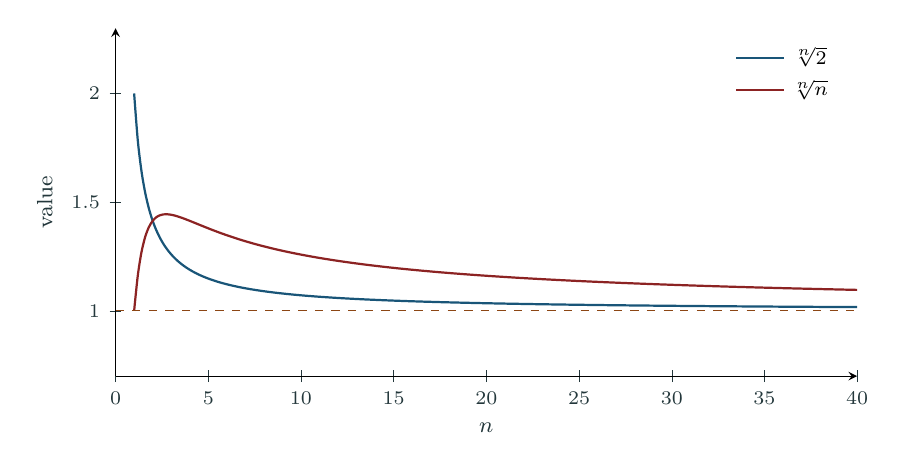
\begin{tikzpicture}
    \begin{axis}[
      width=11cm, height=6cm,
      xmin=0, xmax=40, ymin=0.7, ymax=2.3,
      xlabel={\footnotesize $n$},
      ylabel={\footnotesize value},
      axis lines=left,
      tick style={color=mDarkTeal},
      label style={color=mDarkTeal},
      tick label style={color=mDarkTeal, font=\scriptsize},
      legend style={at={(0.98,0.98)}, anchor=north east, font=\scriptsize, draw=none, fill=none}
    ]
      \addplot[smooth, thick, defcolor, domain=1:40, samples=200]
        {2^(1/x)};
      \addlegendentry{$\sqrt[n]{2}$}
      \addplot[smooth, thick, thmcolor, domain=1:40, samples=200]
        {x^(1/x)};
      \addlegendentry{$\sqrt[n]{n}$}
      \addplot[dashed, mAccent, domain=0:40] {1};
    \end{axis}
  \end{tikzpicture}
  \end{center}

  \vspace{0.2em}
  \begin{center}
    \hl{\emph{Both sequences descend gently toward $1$ as $n$ grows.}}
  \end{center}

  \note{
    Here is a numerical picture of parts "b" and "c". The horizontal
    axis is the index "n" and the vertical axis is the value. The
    blue curve is the "n" th root of 2, an example of part "b". It
    starts above 1 at small "n" and decreases toward 1. The red
    curve is the "n" th root of "n", from part "c". It rises
    briefly because for small "n" it can exceed the blue curve, but
    very quickly it also bends back down toward 1. The orange dashed
    line is the asymptote at value 1, which both curves approach as
    "n" grows.
  }
\end{frame}

% --- Proof of (d): Build 1/3 (setup + binomial lower bound) ---
\begin{frame}{Proof of (d): $n^\alpha / (1+p)^n \to 0$}
  \begin{hlbox}
    \textbf{Setup.} Fix an integer $k$ with $k > \alpha$ and $k > 0$.\\
    \emph{Idea: bound $(1+p)^n$ below by a power of $n$ exceeding $\alpha$.}
  \end{hlbox}

  \vspace{0.4em}
  \begin{proofblock}{Steps (for $n > 2k$)}
    \begin{enumerate}
      \item \textbf{Binomial lower bound.}
        $\displaystyle (1+p)^n \geq \binom{n}{k} p^k = \frac{n(n-1)\cdots(n-k+1)}{k!}\, p^k > \frac{n^k p^k}{2^k k!}.$
    \end{enumerate}
  \end{proofblock}

  \note{
    For part "d", the heart of the argument is to bound the
    exponential 1 plus "p" raised to the "n" th power below by a
    polynomial in "n" of degree higher than alpha. The setup line
    fixes an integer "k" strictly greater than alpha and also
    positive; this "k" is the degree of that polynomial.

    Step 1 expands the exponential via the binomial theorem and
    keeps only the "k" th term, which equals "n" choose "k" times
    "p" to the "k". The binomial coefficient is a product of "k"
    consecutive integers from "n" down to "n" minus "k" plus 1,
    divided by "k" factorial. For "n" exceeding twice "k", each of
    those integers is at least "n" over 2, so the product exceeds
    "n" to the "k" divided by 2 to the "k". This delivers the
    cleaner lower bound on the right.
  }
\end{frame}

% --- Proof of (d): Build 2/3 (+ rearrange ratio) ---
\begin{frame}{Proof of (d): $n^\alpha / (1+p)^n \to 0$}
  \begin{hlbox}
    \textbf{Setup.} Fix an integer $k$ with $k > \alpha$ and $k > 0$.
  \end{hlbox}

  \vspace{0.4em}
  \begin{proofblock}{Steps (for $n > 2k$)}
    \begin{enumerate}
      \item \textbf{Binomial lower bound.} $\displaystyle (1+p)^n > \frac{n^k p^k}{2^k k!}.$
      \item \textbf{Rearrange the ratio.}
        $\displaystyle 0 < \frac{n^\alpha}{(1+p)^n} < \frac{2^k k!}{p^k}\, n^{\alpha - k}.$
    \end{enumerate}
  \end{proofblock}

  \note{
    Step 2 just divides. The numerator is "n" to the alpha, and the
    denominator is bounded below by "n" to the "k" times "p" to the
    "k", divided by 2 to the "k" times "k" factorial. Inverting and
    multiplying gives the bound on the slide: the ratio is less
    than a fixed positive constant times "n" raised to the power
    alpha minus "k". The key point is that alpha minus "k" is
    strictly negative, because we chose "k" larger than alpha. So
    the variable factor is a power of "n" with a negative exponent.
  }
\end{frame}

% --- Proof of (d): Build 3/3 (+ apply (a)) ---
\begin{frame}{Proof of (d): $n^\alpha / (1+p)^n \to 0$}
  \begin{hlbox}
    \textbf{Setup.} Fix an integer $k$ with $k > \alpha$ and $k > 0$.
  \end{hlbox}

  \vspace{0.4em}
  \begin{proofblock}{Steps (for $n > 2k$)}
    \begin{enumerate}
      \item \textbf{Binomial lower bound.} $\displaystyle (1+p)^n > \frac{n^k p^k}{2^k k!}.$
      \item \textbf{Rearrange the ratio.}
        $\displaystyle 0 < \frac{n^\alpha}{(1+p)^n} < \frac{2^k k!}{p^k}\, n^{\alpha - k}.$
      \item \textbf{Apply (a).} Write $\alpha - k = -q$ with $q > 0$. \\
      Then $\displaystyle n^{\alpha - k} = \frac{1}{n^q} \to 0$, so $\displaystyle \frac{n^\alpha}{(1+p)^n} \to 0$. \quad $\Box$
    \end{enumerate}
  \end{proofblock}

  \note{
    Step 3 finishes the proof. Writing alpha minus "k" as the
    negative of a positive number "q", the variable factor "n" to
    the alpha minus "k" is the same as 1 over "n" to the "q",
    which goes to zero by part "a". So the right hand side of the
    bound, a fixed constant times this vanishing factor, goes to
    zero. The squeeze remark applies once more, and the original
    ratio goes to zero. That settles part "d".
  }
\end{frame}

% --- Visual: exponentials beat polynomials (after proof of (d)) ---
\begin{frame}{Picture: Exponentials Beat Polynomials}
  \begin{center}
  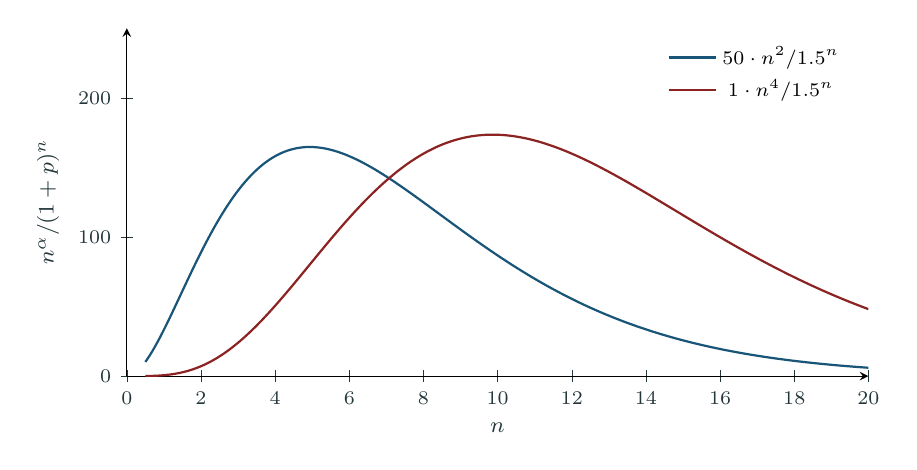
\begin{tikzpicture}
    \begin{axis}[
      width=11cm, height=6cm,
      xmin=0, xmax=20, ymin=0, ymax=250.0,
      xlabel={\footnotesize $n$},
      ylabel={\footnotesize $n^\alpha / (1+p)^n$},
      axis lines=left,
      tick style={color=mDarkTeal},
      label style={color=mDarkTeal},
      tick label style={color=mDarkTeal, font=\scriptsize},
      legend style={at={(0.98,0.98)}, anchor=north east, font=\scriptsize, draw=none, fill=none}
    ]
      \addplot[smooth, thick, defcolor, domain=0.5:20, samples=200]
        {50 * x^2 / (1.5)^x};
      \addlegendentry{$50 \cdot n^2 / 1.5^n$}
      \addplot[smooth, thick, thmcolor, domain=0.5:20, samples=200]
        {x^4 / (1.5)^x};
      \addlegendentry{$1 \cdot n^4 / 1.5^n$}
    \end{axis}
  \end{tikzpicture}
  \end{center}

  \vspace{0.1em}
  \begin{center}
    \hl{\emph{No matter how large $\alpha$ is, the exponential eventually wins.}}
  \end{center}

  \note{
    Here is the picture behind part "d", with "p" set to one half,
    so the denominator is 1.5 to the "n". The horizontal axis is
    the index "n" and the vertical axis is the ratio "n" to the
    alpha over 1.5 to the "n". The blue curve is the case alpha
    equals 2; the red curve is alpha equals 4. The alpha equals 2
    ratio is naturally much smaller, so we scaled the blue curve
    up by a factor of 50 to make the two comparable in one frame;
    the red curve is shown at true size. Both curves tell the same
    story: each rises for a while, reaches a peak, and then
    collapses toward zero. No matter how large alpha is, the
    exponential growth in the denominator eventually overwhelms
    the polynomial growth on top.
  }
\end{frame}

% --- Proof of (e): Build 1/2 (setup) ---
\begin{frame}{Proof of (e): $x^n \to 0$ when $|x| < 1$}
  \begin{proofblock}{Setup: write $|x| = 1/(1+p)$}
    Let $x$ with $|x| < 1$. If $x = 0$, trivially $x^n \to 0$. Otherwise put
    \[
      p \;=\; \frac{1}{|x|} - 1 \;>\; 0,
      \qquad\text{so}\qquad
      |x| \;=\; \frac{1}{1 + p}.
    \]
  \end{proofblock}

  \note{
    Part "e" is a one-line consequence of part "d", but we need to
    set up the right substitution. Suppose the absolute value of "x"
    is strictly less than 1. If "x" is zero, every power is zero,
    and we are done. Otherwise, write the absolute value of "x" as
    1 over 1 plus some positive number "p". This is always possible
    because, by hypothesis, the reciprocal of the absolute value of
    "x" exceeds 1, so subtracting 1 leaves a positive number.
  }
\end{frame}

% --- Proof of (e): Build 2/2 (apply (d) with alpha=0) ---
\begin{frame}{Proof of (e): $x^n \to 0$ when $|x| < 1$}
  \begin{proofblock}{Apply part (d) with $\alpha = 0$}
    Let $x$ with $|x| < 1$. If $x = 0$, trivially $x^n \to 0$. Otherwise put
    \[
      p \;=\; \frac{1}{|x|} - 1 \;>\; 0,
      \qquad\text{so}\qquad
      |x| \;=\; \frac{1}{1 + p}.
    \]
    \[
      |x^n| \;=\; |x|^n \;=\; \frac{1}{(1+p)^n} \;=\; \frac{n^0}{(1+p)^n} \;\to\; 0.
    \]
  Since $|x^n| \to 0$, we have $x^n \to 0$. \quad $\Box$
  \end{proofblock}

  \note{
    The absolute value of "x" to the "n" is 1 over 1 plus "p"
    raised to the "n" th power, which equals "n" to the 0 over 1
    plus "p" raised to the "n" th power. That is exactly the
    expression in part "d" with alpha set to zero. By part "d", it
    goes to zero. Since the absolute value of "x" to the "n" goes
    to zero, "x" to the "n" itself goes to zero. That completes the
    proof of Theorem 3.20.
  }
\end{frame}

}

{
\usebackgroundtemplate{%
  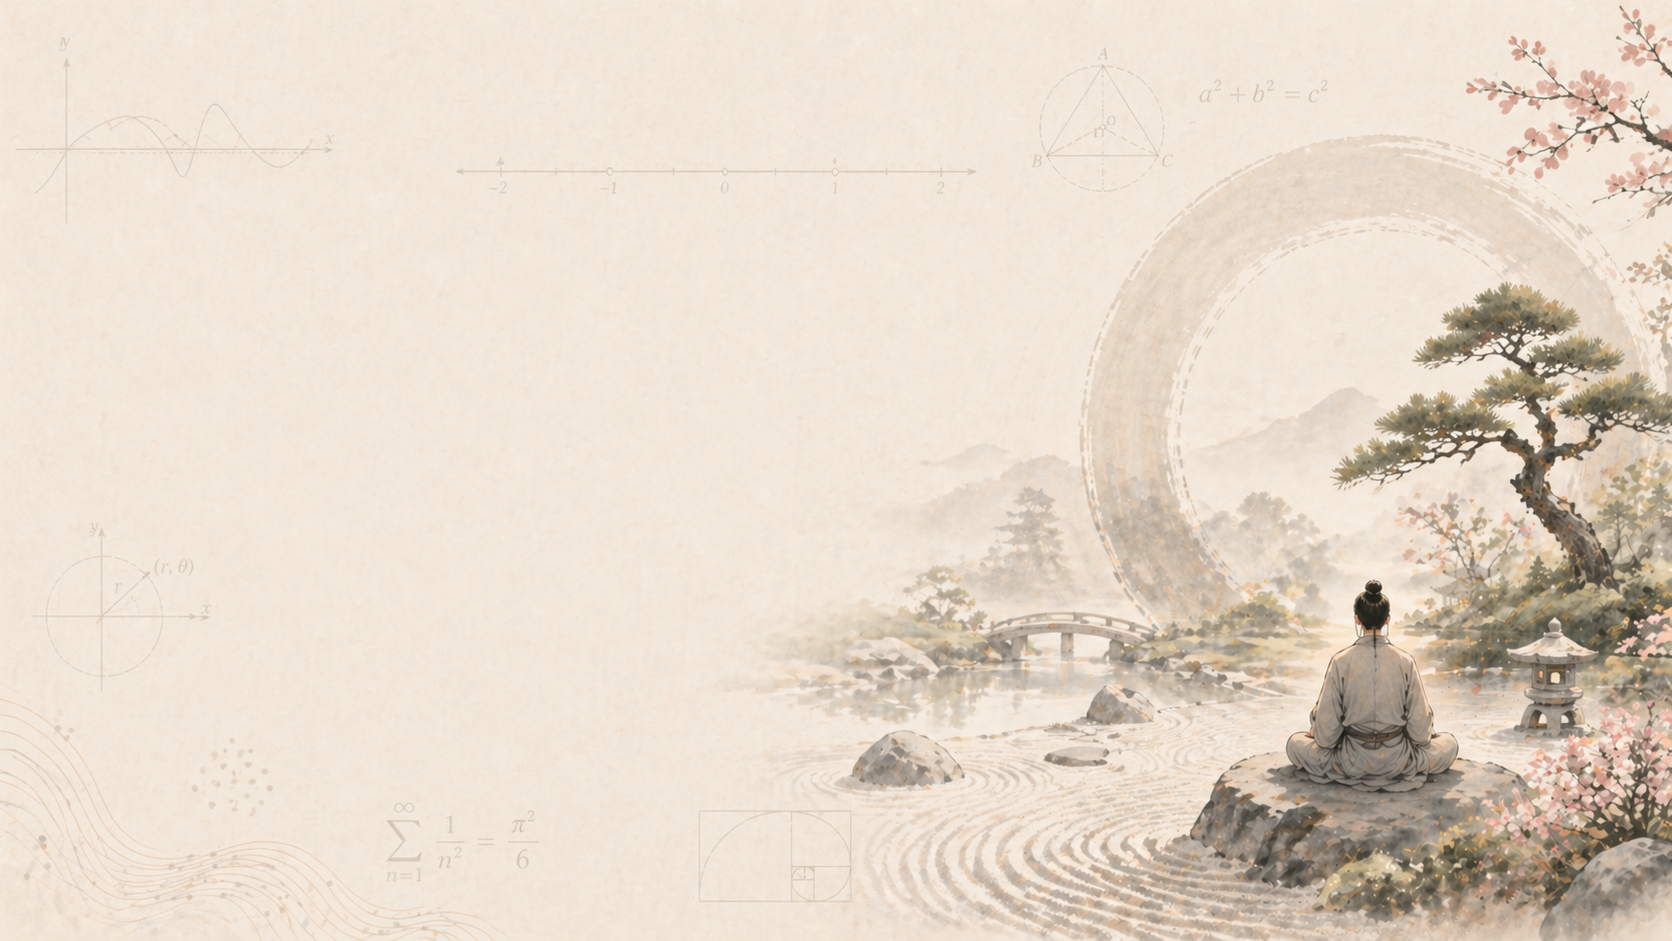
\includegraphics[width=\paperwidth,height=\paperheight,keepaspectratio=false]{chapter_03_bg_06.png}%
}
% =============================================================================
% SUMMARY
% =============================================================================
\section{Summary}

% --- Summary: Build 1/6 ---
\begin{frame}{Summary}
  \begin{hlbox}
    \textbf{Key takeaways from this section:}
    \begin{itemize}
      \item \alert{Squeeze remark:} $0 \leq x_n \leq s_n$ and $s_n \to 0$ $\Longrightarrow$ $x_n \to 0$
    \end{itemize}
  \end{hlbox}

  \note{
    Let us recap. The first of our two tools is the squeeze: if a
    sequence is sandwiched between zero and another sequence that
    goes to zero, then it goes to zero too. That simple remark is
    the engine behind every proof.
  }
\end{frame}
 
% --- Summary: Build 2/6 ---
\begin{frame}{Summary}
  \begin{hlbox}
    \textbf{Key takeaways from this section:}
    \begin{itemize}
      \item \alert{Squeeze remark:} $0 \leq x_n \leq s_n$ and $s_n \to 0$ $\Longrightarrow$ $x_n \to 0$
      \item \alert{Binomial theorem:} $(a+b)^n = \sum_{k=0}^{n} \binom{n}{k} a^{n-k} b^k$
    \end{itemize}
  \end{hlbox}

  \note{
    The second tool is the binomial theorem. It expands "a" plus
    "b" to the "n" th power as a sum of binomial coefficient terms.
    We proved it by induction, and the key identity driving that
    induction was Pascal's rule, which says "n" plus 1 choose "k"
    equals "n" choose "k" plus "n" choose "k" minus 1. The binomial
    theorem is what supplies the bounds we then feed into the
    squeeze.
  }
\end{frame}

% --- Summary: Build 3/6 ---
\begin{frame}{Summary}
  \begin{hlbox}
    \textbf{Key takeaways from this section:}
    \begin{itemize}
      \item \alert{Squeeze remark:} $0 \leq x_n \leq s_n$ and $s_n \to 0$ $\Longrightarrow$ $x_n \to 0$
      \item \alert{Binomial theorem:} $(a+b)^n = \sum_{k=0}^{n} \binom{n}{k} a^{n-k} b^k$
      \item \alert{Thm. 3.20 (a):} $\dfrac{1}{n^p} \to 0$ for $p > 0$
    \end{itemize}
  \end{hlbox}

  \note{
    Part "a" of Theorem 3.20 says that 1 over "n" to the "p" tends
    to zero for every positive power "p". This is the workhorse for
    everything that follows.
  }
\end{frame}

% --- Summary: Build 4/6 ---
\begin{frame}{Summary}
  \begin{hlbox}
    \textbf{Key takeaways from this section:}
    \begin{itemize}
      \item \alert{Squeeze remark:} $0 \leq x_n \leq s_n$ and $s_n \to 0$ $\Longrightarrow$ $x_n \to 0$
      \item \alert{Binomial theorem:} $(a+b)^n = \sum_{k=0}^{n} \binom{n}{k} a^{n-k} b^k$
      \item \alert{Thm. 3.20 (a):} $\dfrac{1}{n^p} \to 0$ for $p > 0$
      \item \alert{Thm. 3.20 (b), (c):} $\sqrt[n]{p} \to 1$ for $p > 0$;\quad $\sqrt[n]{n} \to 1$
    \end{itemize}
  \end{hlbox}

  \note{
    Parts "b" and "c" record two perhaps-surprising root limits.
    The "n" th root of a positive constant tends to 1, and so does
    the "n" th root of "n" itself. Both proofs followed the same
    pattern: write the root as 1 plus a small correction, bound the
    correction by the binomial theorem, and squeeze.
  }
\end{frame}

% --- Summary: Build 5/6 ---
\begin{frame}{Summary}
  \begin{hlbox}
    \textbf{Key takeaways from this section:}
    \begin{itemize}
      \item \alert{Squeeze remark:} $0 \leq x_n \leq s_n$ and $s_n \to 0$ $\Longrightarrow$ $x_n \to 0$
      \item \alert{Binomial theorem:} $(a+b)^n = \sum_{k=0}^{n} \binom{n}{k} a^{n-k} b^k$
      \item \alert{Thm. 3.20 (a):} $\dfrac{1}{n^p} \to 0$ for $p > 0$
      \item \alert{Thm. 3.20 (b), (c):} $\sqrt[n]{p} \to 1$ for $p > 0$;\quad $\sqrt[n]{n} \to 1$
      \item \alert{Thm. 3.20 (d):} \emph{exponentials beat polynomials}: $\dfrac{n^\alpha}{(1+p)^n} \to 0$
    \end{itemize}
  \end{hlbox}

  \note{
    Part "d" is the most powerful entry on the list. It says that
    exponential growth in the denominator overwhelms any
    polynomial-style growth in the numerator. This is the slogan to
    keep in mind: exponentials beat polynomials. It will show up
    again every time we compare growth rates.
  }
\end{frame}

% --- Summary: Build 6/6 ---
\begin{frame}{Summary}
  \begin{hlbox}
    \textbf{Key takeaways from this section:}
    \begin{itemize}
      \item \alert{Squeeze remark:} $0 \leq x_n \leq s_n$ and $s_n \to 0$ $\Longrightarrow$ $x_n \to 0$
      \item \alert{Binomial theorem:} $(a+b)^n = \sum_{k=0}^{n} \binom{n}{k} a^{n-k} b^k$
      \item \alert{Thm. 3.20 (a):} $\dfrac{1}{n^p} \to 0$ for $p > 0$
      \item \alert{Thm. 3.20 (b), (c):} $\sqrt[n]{p} \to 1$ for $p > 0$;\quad $\sqrt[n]{n} \to 1$
      \item \alert{Thm. 3.20 (d):} \emph{exponentials beat polynomials}: $\dfrac{n^\alpha}{(1+p)^n} \to 0$
      \item \alert{Thm. 3.20 (e):} $x^n \to 0$ for $|x| < 1$ (geometric decay)
    \end{itemize}
  \end{hlbox}

  \note{
    Finally part "e" gives the geometric decay we will use all the
    time: powers of any number whose absolute value is strictly less
    than 1 collapse to zero. This will be the backbone of the
    geometric series and the root and ratio tests.
  }
\end{frame}

% --- Coming up next ---
\begin{frame}{Coming Up Next}
  \begin{hlbox}
    \textbf{Next section: Series}
    \begin{itemize}
      \item Partial sums and what it means for a series to converge
      \item Tests for convergence (Cauchy criterion, comparison, root, ratio)
      \item Many of these tests will lean on the five limits we just established
    \end{itemize}
  \end{hlbox}

  \note{
    Coming up next we turn from sequences to series. We define
    what it means for an infinite sum to converge, and we develop
    the standard tests: the Cauchy criterion for series, the
    comparison test, the root test, and the ratio test. Several of
    these tests lean directly on the five special limits we just
    established. So even though this section was short, its results
    will be in play for the rest of the chapter. See you in the
    next section.
  }
\end{frame}
}

\end{document}
